\section{Matematička formulacija i konceptualni model problema}
\label{chap:model_problema}
Nakon pregleda teorijskih osnova, ovo poglavlje posvećeno je formalnoj definiciji problema optimizacije projektnog portfelja. Cilj je prevesti realni poslovni problem u precizan matematički i konceptualni model na koji se mogu primijeniti računalne metode optimizacije. U nastavku se detaljno opisuju ulazni entiteti, varijable odluke, primijenjena resursna ograničenja te jedno-kriterijski i više-kriterijski ciljevi koji su korišteni u kasnijoj eksperimentalnoj evaluaciji.
\subsection{Definicija skupa aktivnosti i varijabli odluke}
Problem se definira kao odabir optimalnog podskupa (portfelja) aktivnosti iz većeg, unaprijed definiranog skupa dostupnih aktivnosti. U korijenu problema nalazi se skup od $n$ potencijalnih projektnih aktivnosti, $A=\{a_1, a_2, ..., a_n\}$ iz kojeg je potrebno odabrati optimalan podskup (portfelj). Ovakav problem odabira predstavlja čest izazov u praksi projektnog menadžmenta \cite{PMI2021, Kerzner2017}.  Svaka aktivnost $a_i \in A$ opisana je s tri ključna atributa koji definiraju njezin trošak, cijenu i rizik.

 Odabir ovih specifičnih atributa temelji se na fundamentalnim principima upravljanja projektima, koji uvijek balansiraju između investicije, očekivanog povrata i inherentnog rizika. Prvi je trošak ($c_i$), koji predstavlja količinu budžeta ili drugih resursa potrebnih za izvođenje aktivnosti. On je primarni faktor ograničenja. Drugi atribut je vrijednost ($v_i$), definirana kao povrat na investiciju (ROI).  Ona kvantificira korist ili profit koji se ostvaruje uspješnim završetkom aktivnosti i predstavlja primarni cilj maksimizacije. Treći, ključni atribut je nesigurnost trajanja. U ovom modelu, trajanje se ne definira kao jedna deterministička vrijednost već kao stohastička varijabla opisana s tri točke procjene: optimističnom ($T_o$), najvjerojatnijom ($T_m$) i pesimističnom ($T_p$). Ove procjene služe kao parametri za Trokutastu distribuciju unutar Monte Carlo simulacije, čime se rizik trajanja uvodi kao integralni dio modela. Ovakav pristup izravno usvaja najbolje prakse iz domene upravljanja projektnim rizikom, poput PERT metodologije, kako bi se u model ugradila realistična slika neizvjesnosti.
S obzirom na navedene atribute, temeljni zadatak optimizacije je definirati binarni vektor odluke $x=(x_1, x_2, ..., x_n)$, gdje $x_i \in \{0,1\}$. Vrijednost $x_i=1$ označava da je aktivnost $a_i$ odabrana za uključivanje u portfelj, dok $x_i=0$ označava da se aktivnost ne izvodi. Ovaj vektor odluke je upravo ono što genetski algoritam nastoji optimizirati.

\subsection{Resursna ograničenja modela}
Svaki realni projekt podložan je ograničenjima. U ovom modelu implementirano je ključno i najčešće ograničenje u upravljanju portfeljem: ograničenje budžeta ($B_{max}$). Formalno, ovo ograničenje pripada klasi linearnih nejednakosti koje su standard u području cjelobrojnog programiranja (\textit{Integer Programming}), čiji je problem ruksaka klasičan primjer \cite{Glover1986}. Prema ovom pravilu, ukupni zbroj troškova svih odabranih aktivnosti ne smije prelaziti ukupno raspoloživi budžet. Upravo ovo ograničenje čini problem optimizacijski izazovnim; bez njega, trivijalno rješenje bilo bi odabrati sve profitabilne aktivnosti. Dakle, ovo ograničenje odgovara klasičnoj formulaciji problema ruksaka \texttt{Knapsack problem}\cite{Kellerer2004} i matematički se izražava kao:
$$
\sum_{i=1}^n c_i x_i \leq B_{max}
$$
Vrijedi napomenuti da ukupno trajanje portfelja nije tretirano kao strogo ograničenje, već kao izlazna metrika performansi i cilj za minimizaciju. Ova metodološka odluka je ključna, jer omogućuje modelu da provodi \textbf{analizu kompromisa (trade-off analysis)}, sličnu onoj u teoriji financijskih portfelja. Umjesto postavljanja proizvoljnog roka i rigidnog odbacivanja svih rješenja koja ga prelaze, ovakav pristup omogućuje algoritmu da pronađe rješenja koja su možda malo duža, ali značajno profitabilnija, pružajući donositelju odluke puno bogatiji set informacija. To je u skladu s modernim praksama upravljanja projektnom nesigurnošću, gdje je cilj razumjeti i upravljati rizikom, a ne ga rigidno ograničiti \cite{Smith2014}.

\subsection{Specifikacija optimizacijskih ciljeva}
Ciljna funkcija (ili funkcija pogodnosti) je matematički izraz koji kvantificira kvalitetu pojedinog rješenja (portfelja). U skladu s eksperimentalnim dizajnom, definirana su i analizirana dva različita optimizacijska cilja.

Prvi, \textbf{jedno-kriterijski cilj}, predstavlja klasični financijski pristup usmjeren isključivo na maksimizaciju dobiti često nazivan pristupom "maksimizacije vrijednosti za dioničare". Ovaj pristup odgovara GA (samo ROI) modelu, a njegova ciljna funkcija $f(\mathbf{x})$ je maksimizacija ukupnog zbroja ROI vrijednosti odabranih aktivnosti, uz poštivanje ograničenja budžeta. Ovakav tip optimizacijskog cilja čest je u primjeni genetskih algoritama na probleme alokacije resursa \cite{Goldberg1989}, a formalno se zapisuje kao:
$$ \text{maksimizirati } f(\mathbf{x}) = \sum_{i=1}^n v_i x_i $$

S druge strane, \textbf{više-kriterijski cilj} predstavlja srž ovog istraživanja i odgovara naprednom hibridnom GA+MC (NSGA-II) modelu. Realnost upravljanja projektima jest inherentno više-kriterijska. Uspjeh projekta se rijetko mjeri samo jednim pokazateljem, već balansom između troškova, vremena, opsega i kvalitete \cite{PMI2021}. Model to aproksimira kroz dva ključna, suprotstavljena cilja: maksimizaciju profita (ROI) i minimizaciju rizika (procijenjeno trajanje). U ovom pristupu istovremeno se optimiziraju dva suprotstavljena cilja: maksimizacija profita i minimizacija rizika. Definiramo dvije ciljne funkcije: $f_1(\mathbf{x})$ za ukupni ROI i $f_2(\mathbf{x})$ za procijenjeno trajanje. Više-kriterijski optimizacijski problem tada se može formalno zapisati kao:
$$ \text{maksimizirati } \mathbf{F}(\mathbf{x}) = (f_1(\mathbf{x}), -f_2(\mathbf{x})) $$
gdje je $f_1(\mathbf{x})=\sum_{i=1}^n v_i x_i$, a $f_2(\mathbf{x})=E[T(\mathbf{x})]$.
Negativni predznak ispred $f_2$ koristi se jer je standardna konvencija maksimizirati sve ciljeve. Budući da poboljšanje jednog cilja često degradira drugi, ovaj pristup ne traži jedno "najbolje" rješenje, već skup optimalnih kompromisnih rješenja, poznat kao Paretov front. Svako rješenje na Paretovom frontu je takvo da se niti jedan cilj (u ovom slučaju ROI ili trajanje) ne može poboljšati bez da se drugi cilj istovremeno pogorša. Time Paretov front predstavlja "granicu efikasnosti" i nudi donositelju odluke ne jedno rješenje, već cijeli spektar strateških opcija – od onih s maksimalnim profitom uz veći rizik trajanja, do onih s minimalnim rizikom uz manji profit \cite{Deb2002, Goldberg1989}. Za pronalaženje ovog skupa korišten je renomirani NSGA-II algoritam, detaljno opisan u Poglavlju 2.
\subsection{Konceptualni prikaz i značaj modela}

Konceptualni model problema, koji objedinjuje sve prethodno opisane elemente, prikazan je na Slici \ref{fig:konceptualni_model}. Dijagram ilustrira proces kao sustav s jasno definiranim ulazima, procesom obrade i izlazima. \textbf{Ulaz} u sustav čini cjelokupni skup dostupnih aktivnosti sa svim njihovim atributima (trošak, ROI, procjene trajanja). \textbf{Proces obrade} predstavlja optimizacijski algoritam (genetski algoritam), koji je vođen definiranim \textbf{ciljevima} (maksimizacija ROI-a i/ili minimizacija trajanja) i sputan zadanim \textbf{ograničenjem} (budžet). Algoritam sustavno pretražuje prostor mogućih kombinacija (svih mogućih vektora x) kako bi kao \textbf{izlaz} generirao optimalni portfelj – podskup aktivnosti koji najbolje zadovoljava postavljene kriterije.
\begin{figure}[H]
    \centering
    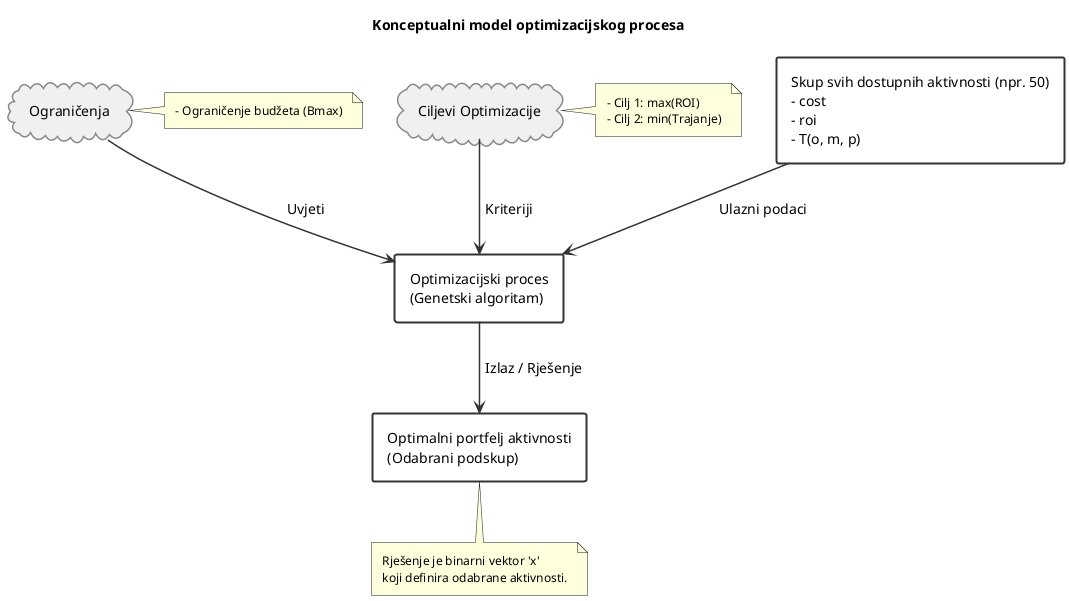
\includegraphics[width=0.9\textwidth]{slike/model_problema.png}
    \caption{Konceptualni model problema optimizacije portfelja projektnih aktivnosti.(Izrada autora)}
    \label{fig:konceptualni_model}
\end{figure}
Ovaj proces formalizacije ključan je korak koji premošćuje jaz između apstraktnog poslovnog problema i konkretnog računarskog rješenja. Precizna definicija ulaza, ograničenja i ciljeva služi kao temelj na kojem se grade i primjenjuju optimizacijske metode. Za genetski algoritam, ovaj model definira "pravila igre": binarni vektor odluke ($x$) postaje struktura kromosoma, optimizacijski ciljevi postaju funkcija pogodnosti koja vodi evoluciju, a ograničenje budžeta definira granice valjanog prostora rješenja \cite{Mitchell1998}.
Istovremeno, model pruža nužan okvir za Monte Carlo simulaciju. Stohastički atributi aktivnosti ($T_o$, $T_m$, $T_p$) služe kao direktni ulazni parametri za simulacijski modul. Zauzvrat, Monte Carlo simulacija "obogaćuje" model izračunavanjem vrijednosti za ključni cilj – očekivano trajanje portfelja ($E[T(\mathbf{x})]$) – čime se kvantificira rizik.
Na taj način, formalni model uspostavlja sinergijski odnos između optimizacije i simulacije. Genetski algoritam predlaže visokokvalitetne kandidate za rješenja, dok Monte Carlo simulacija procjenjuje njihovu robusnost u uvjetima nesigurnosti \cite{Rubinstein2016}. Time je postavljen čvrst temelj za praktičnu implementaciju opisanu u sljedećem poglavlju, te za eksperimentalnu evaluaciju koja slijedi nakon toga, s konačnim ciljem dobivanja rješenja koja nisu samo profitabilna, već i pouzdana.
